\documentclass[mathserif]{beamer}
\usepackage{graphicx}
\usepackage{epstopdf}
\usecolortheme{dove}

\title{Moving Target Indicators}
\author{Swrangsar Basumatary (09d07040) \\ Chakradhar Thallapaka (09007046)}
\institute{Department of Electrical Engineering \\ IIT Bombay, Powai}
\date{April 25, 2014}

    
\begin{document}
    \frame{\titlepage}
    
    \begin{frame}{Single Delay Line Cancelers}
    	\begin{figure}[h]
		\centering
		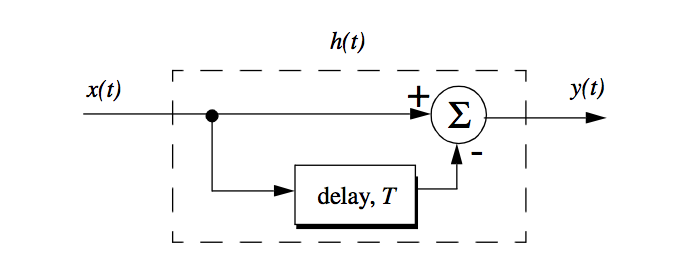
\includegraphics[width=\linewidth]{singleDLC} 
		\caption{Single delay line canceler}
	\end{figure}
		\tiny{Source: Bassem R.~Mahafza. \emph{Radar Systems Analysis and Design Using MATLAB\textsuperscript{\textregistered}}. Chapman \& Hall/CRC, 2000.}

    \end{frame}
    
    
    \begin{frame}{Single Delay Line Cancelers}
   	\begin{align}
    	 h(t) & = \delta(t) - \delta(t-T) \nonumber \\
    	 H(\omega) & = 1 - e^{-j\omega T} \nonumber \\
    	 |H(\omega)|^2 & = H(\omega)H^*(\omega) \nonumber \\
    	 & = (1 - e^{-j\omega T})(1 - e^{j\omega T}) \nonumber \\
    	 & = 2(1-cos\omega T) \nonumber \\
    	 & = 4(sin(\omega T/2))^2 \nonumber
    	\end{align}
    	
    	\vfill
    	\tiny{Source: Bassem R.~Mahafza. \emph{Radar Systems Analysis and Design Using MATLAB\textsuperscript{\textregistered}}. Chapman \& Hall/CRC, 2000.}

    \end{frame}
    
    
    \begin{frame}{Double Delay Line Cancelers}
	\begin{figure}[h]
		\centering
		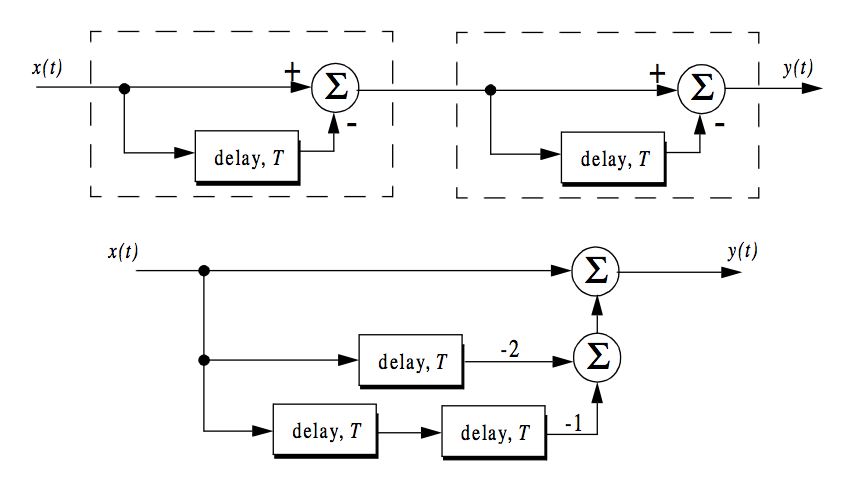
\includegraphics[width=\linewidth]{doubleDLC} 
		\caption{Two configurations for a double delay line canceler}
	\end{figure}
    	\tiny{Source: Bassem R.~Mahafza. \emph{Radar Systems Analysis and Design Using MATLAB\textsuperscript{\textregistered}}. Chapman \& Hall/CRC, 2000.}

    \end{frame}
    
    
    \begin{frame}{Double Delay Line Cancelers}
      \begin{align}
       h(t) & = \delta(t) - 2\delta(t-T) + \delta(t-2T) \nonumber \\
       |H(\omega)|^2 & = |H_1(\omega)|^2|H_1(\omega)|^2 \nonumber \\
       & where~ |H_1(\omega)|^2 = 4(sin(\omega T/2))^2 \nonumber \\
       |H(\omega)|^2 & = 16\left(sin\left(\omega\frac{T}{2}\right)\right)^4 \nonumber
      \end{align}

      \vfill
    	\tiny{Source: Bassem R.~Mahafza. \emph{Radar Systems Analysis and Design Using MATLAB\textsuperscript{\textregistered}}. Chapman \& Hall/CRC, 2000.}

    \end{frame}



    \begin{frame}{Delay Line Cancelers}
    	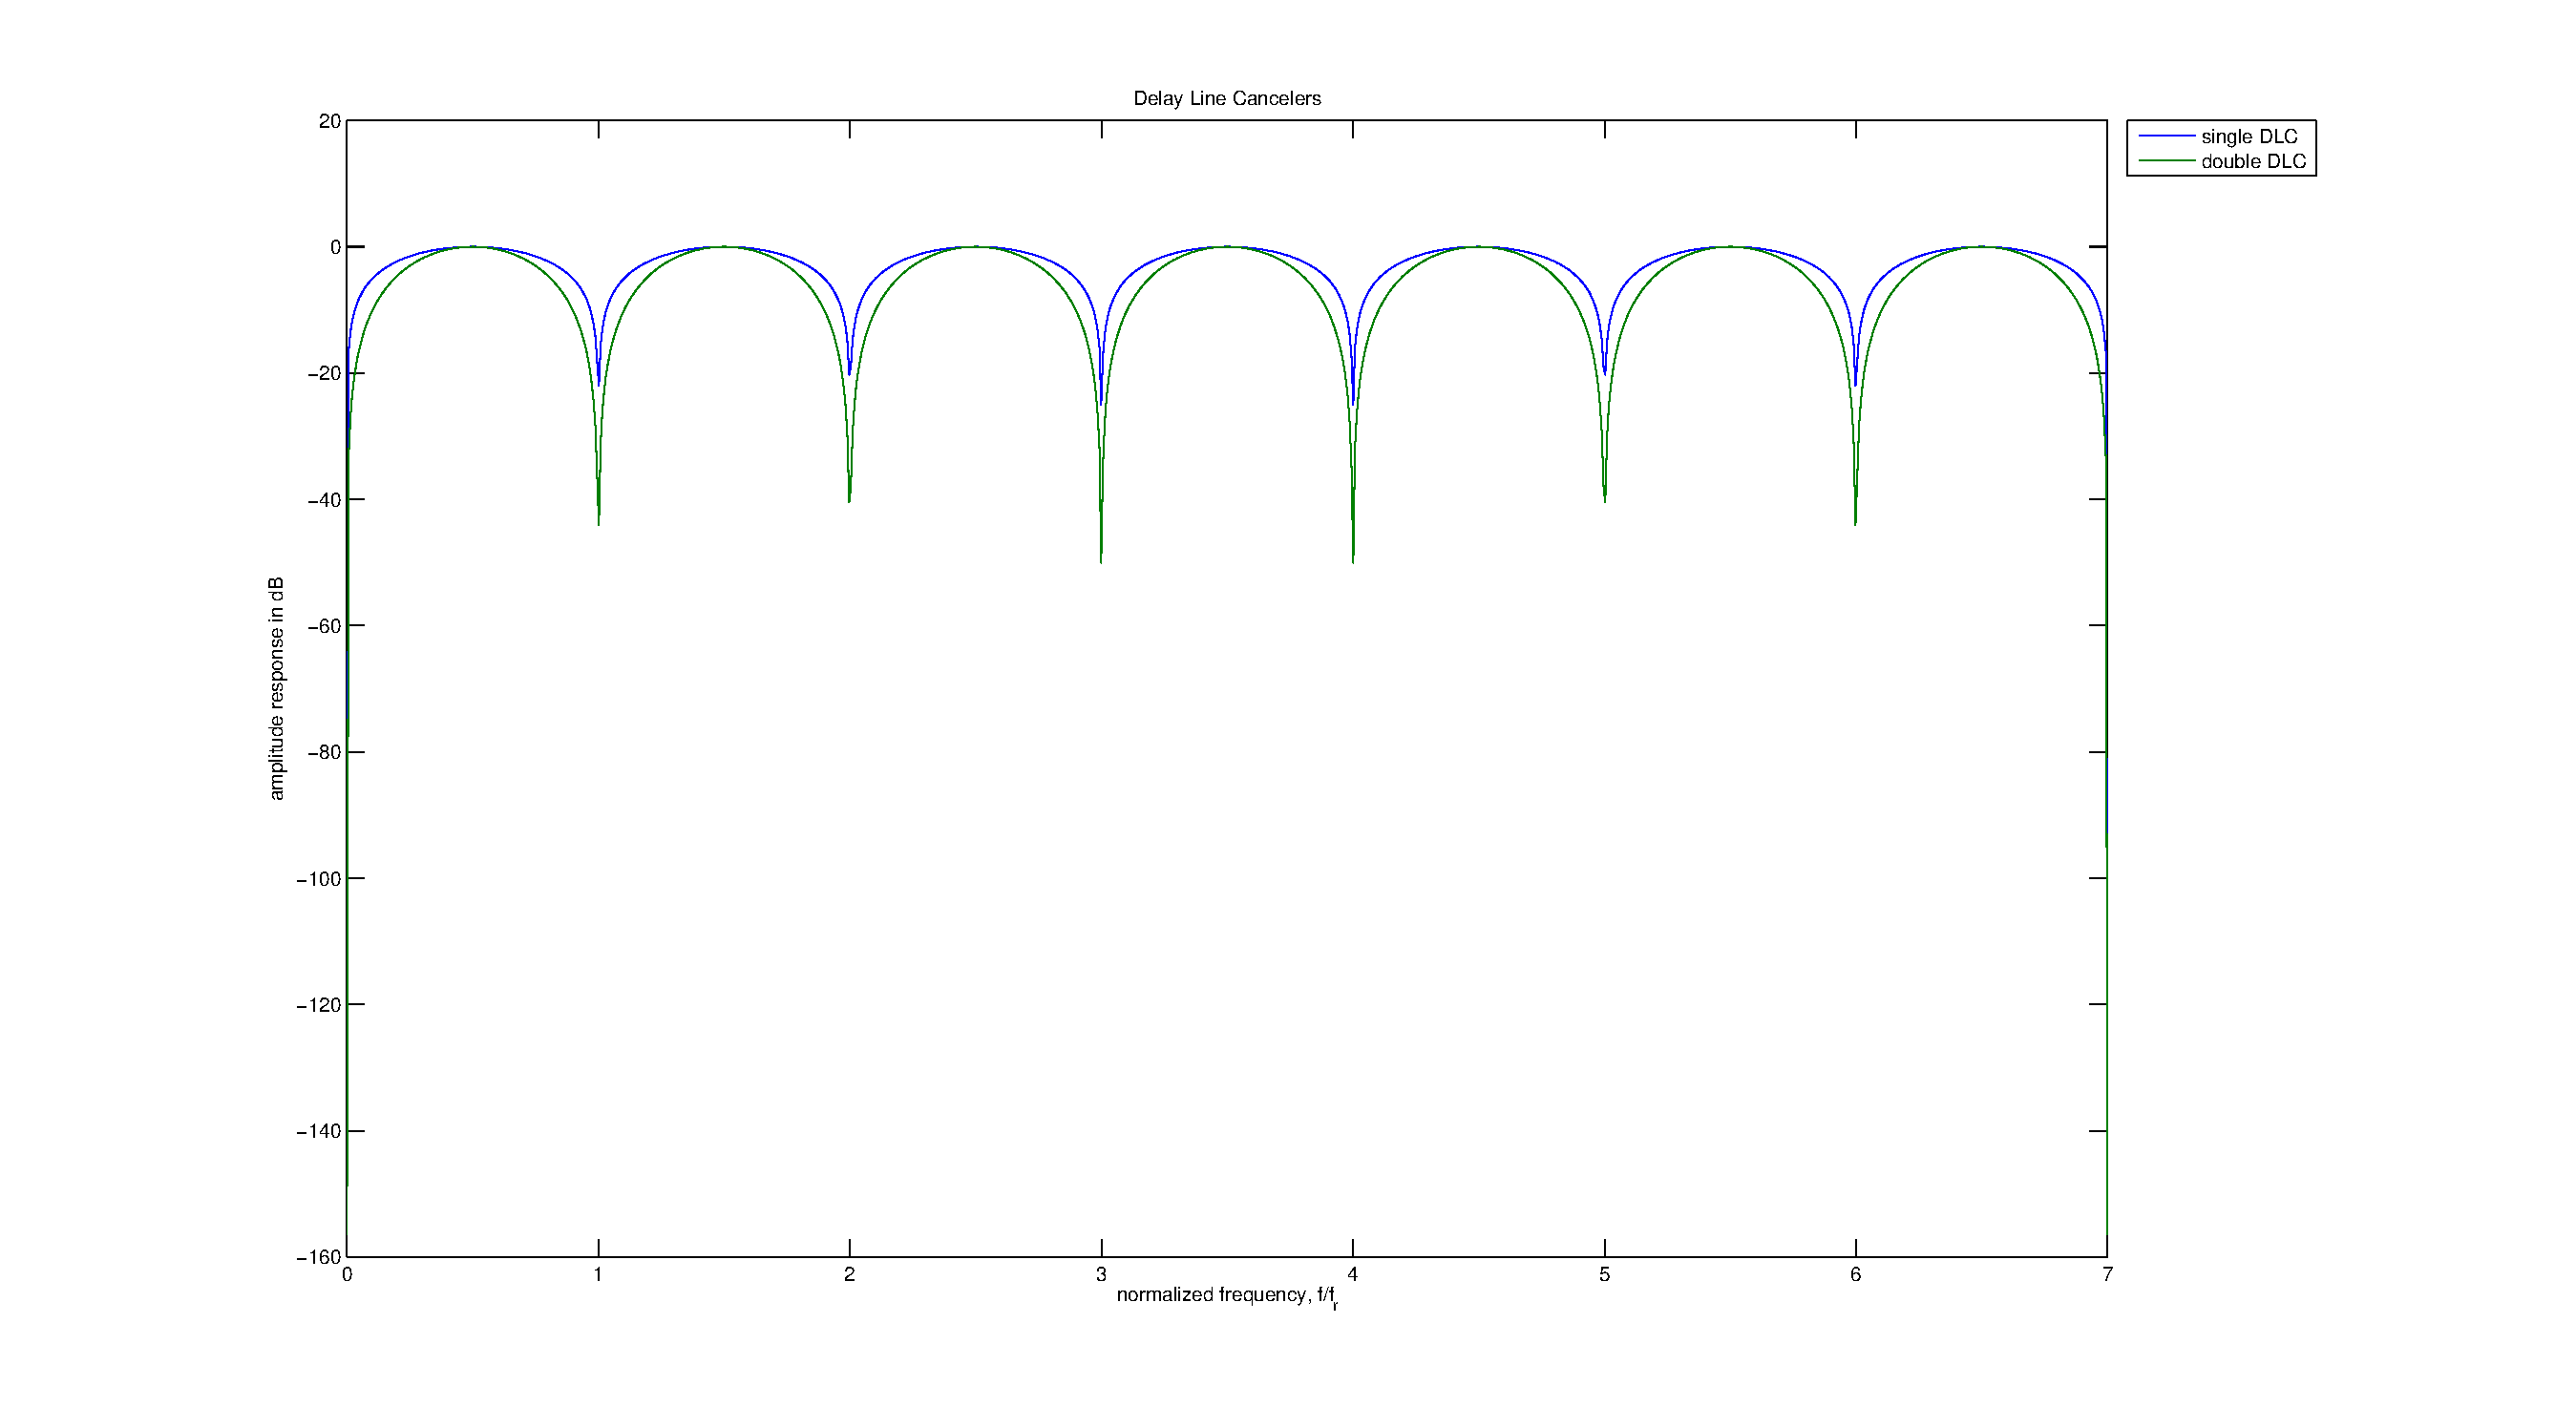
\includegraphics[width=\linewidth]{delayLineCancelers}
    \end{frame}
    
    
    
    \begin{frame}{Delay Lines with Feedback}
	\begin{figure}[h]
		\centering
		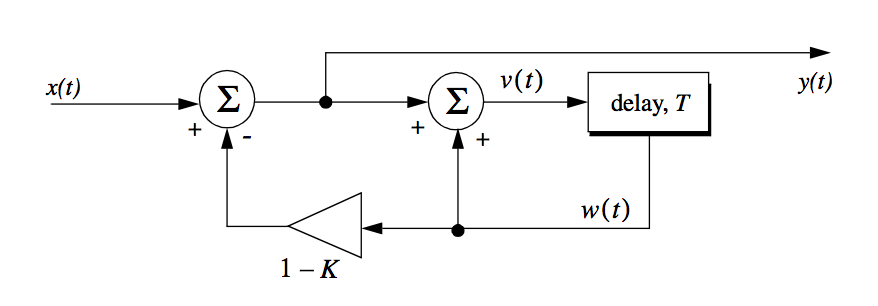
\includegraphics[width=\linewidth]{feedbackDLC} 
		\caption{MTI recursive filter}
	\end{figure}
    	\tiny{Source: Bassem R.~Mahafza. \emph{Radar Systems Analysis and Design Using MATLAB\textsuperscript{\textregistered}}. Chapman \& Hall/CRC, 2000.}
    \end{frame}
    
    
    
    \begin{frame}{Delay Lines with Feedback}
      \begin{align}
      H(z) & = \frac{1 - z^{-1}}{1-Kz^{-1}} \nonumber \\
      |H(z)|^2 & = \frac{(1-z^{-1})(1-z)}{(1-Kz^{-1})(1-Kz)} \nonumber \\
      & = \frac{2-(z+z^{-1})}{(1+K^2)-K(z+z^{-1})} \nonumber \\
      \left|{H(e^{j\omega T})}\right|^2 & = \frac{2(1-cos\omega T)}{(1+K^2)-2Kcos(\omega T)} \nonumber
      \end{align}
      \vfill
    	\tiny{Source: Bassem R.~Mahafza. \emph{Radar Systems Analysis and Design Using MATLAB\textsuperscript{\textregistered}}. Chapman \& Hall/CRC, 2000.}

    \end{frame}
    
    
    \begin{frame}{Delay Lines with Feedback}
      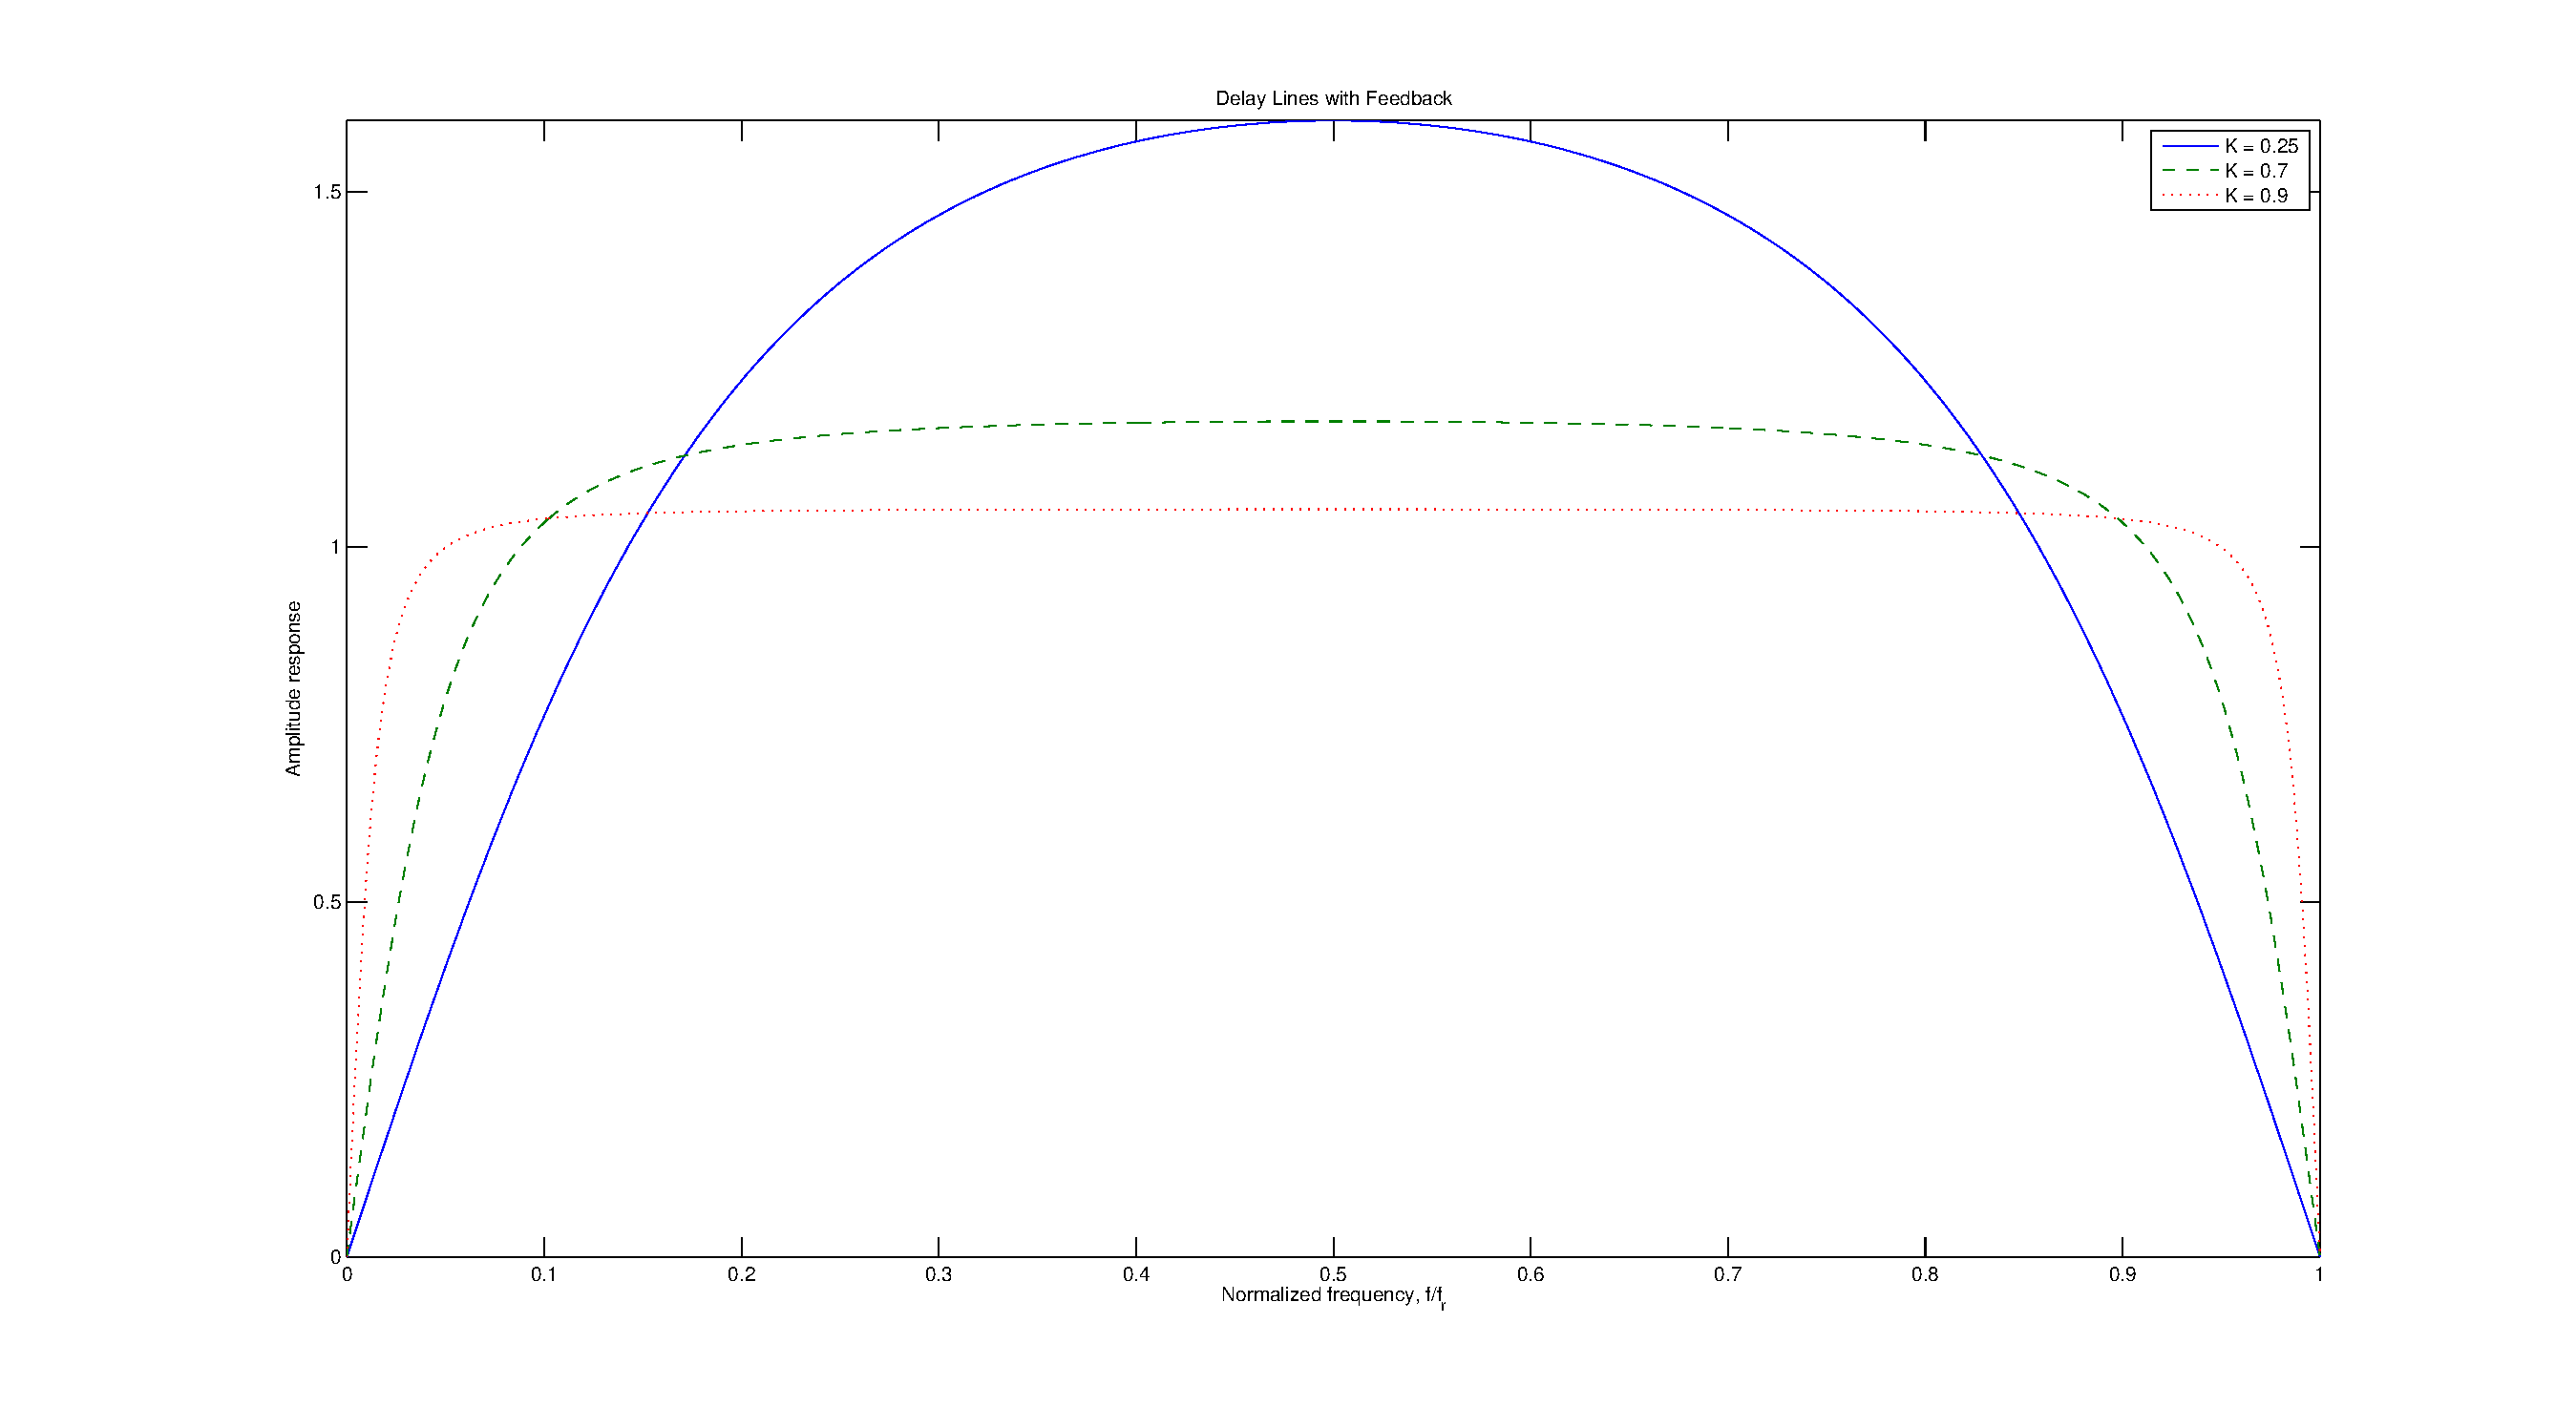
\includegraphics[width=\linewidth]{dlFeedback}
      \tiny{Source: Bassem R.~Mahafza. \emph{Radar Systems Analysis and Design Using MATLAB\textsuperscript{\textregistered}}. Chapman \& Hall/CRC, 2000.}
    \end{frame}
   
    
    \begin{frame}{PRF Staggering 4/5}
	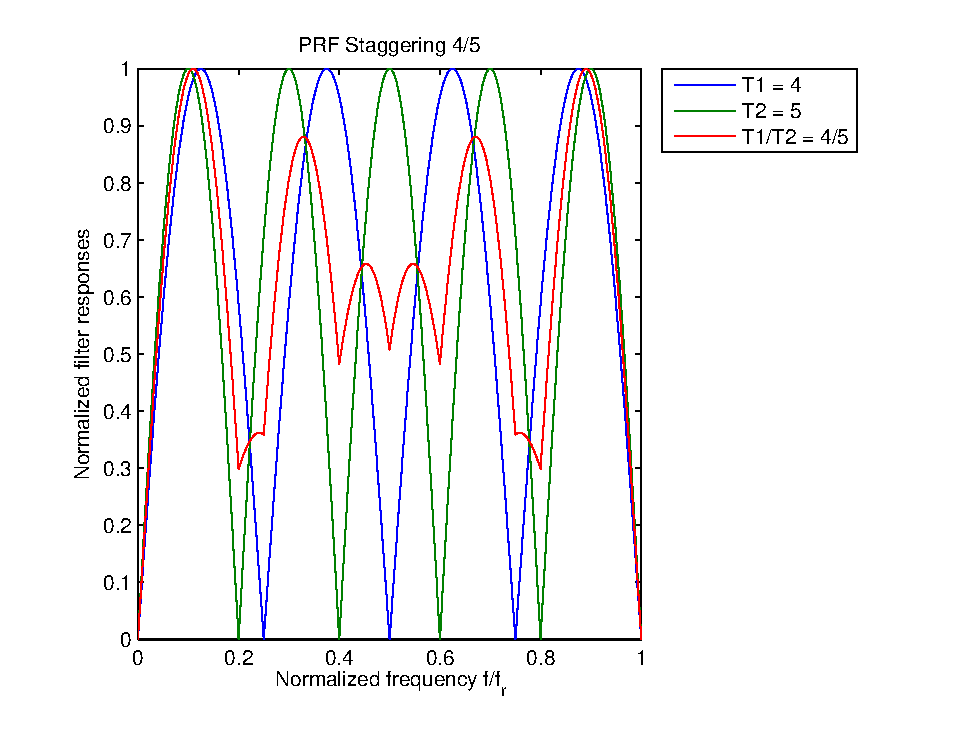
\includegraphics[width=\linewidth]{prfStaggering4_5} \\
	\tiny{Source: Bassem R.~Mahafza. \emph{Radar Systems Analysis and Design Using MATLAB\textsuperscript{\textregistered}}. Chapman \& Hall/CRC, 2000.}
    \end{frame}
    
    
    \begin{frame}{PRF Staggering 33/34}
    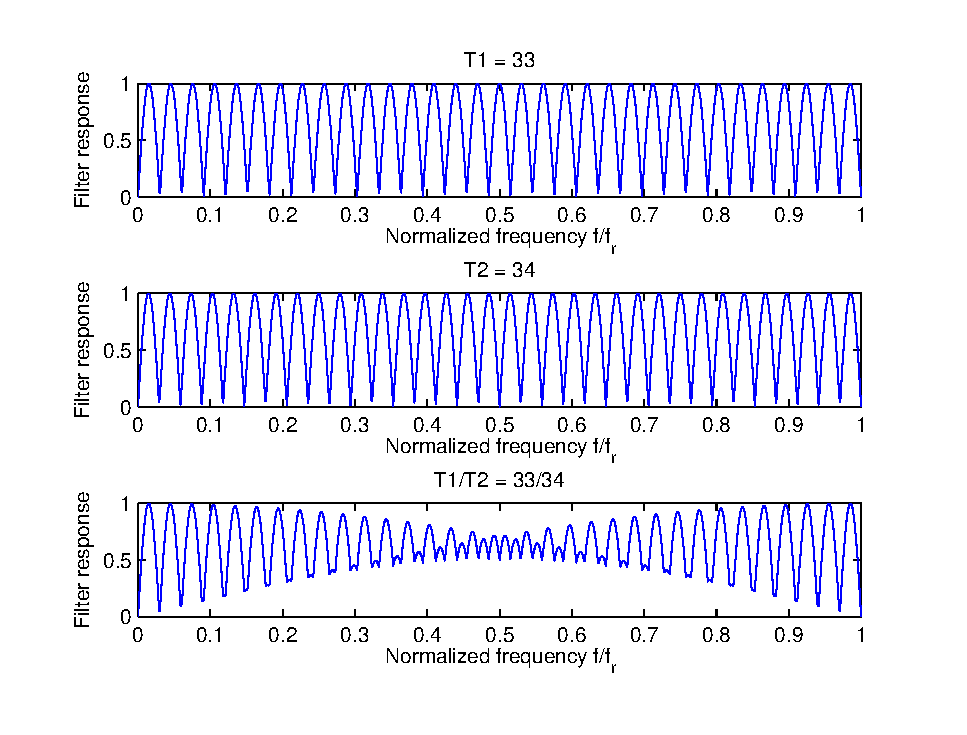
\includegraphics[width=\linewidth]{prfStaggering33_34} \\
      \tiny{Source: Bassem R.~Mahafza. \emph{Radar Systems Analysis and Design Using MATLAB\textsuperscript{\textregistered}}. Chapman \& Hall/CRC, 2000.}
    \end{frame}
    
   
    \begin{frame}{PRF Staggering 63/64}
    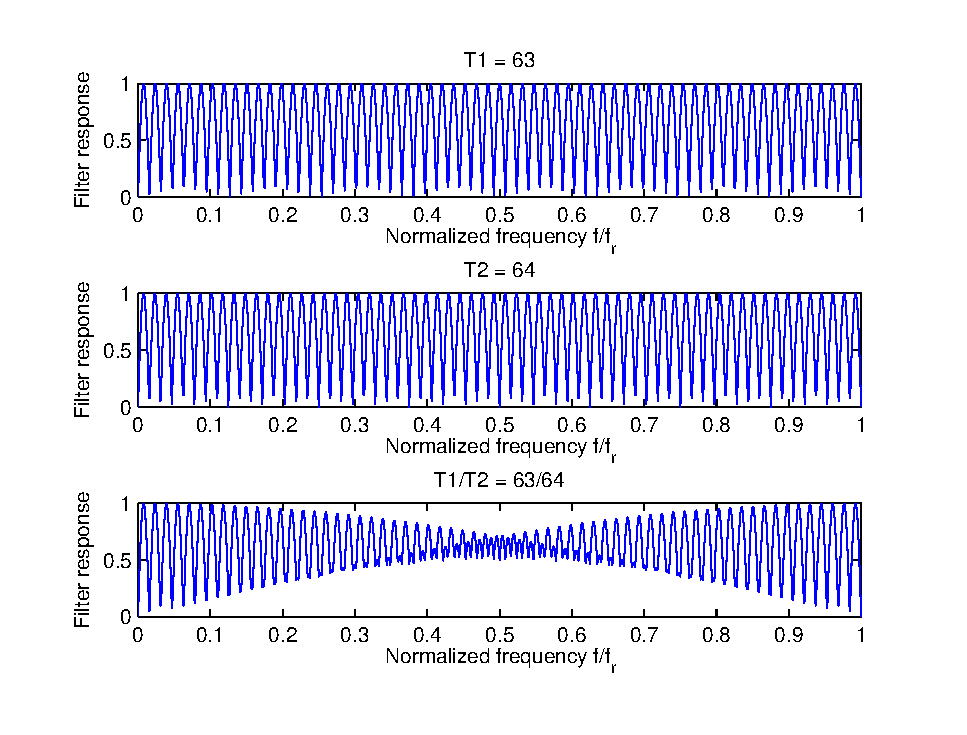
\includegraphics[width=\linewidth]{prfStaggering63_64} \\
      \tiny{Source: Bassem R.~Mahafza. \emph{Radar Systems Analysis and Design Using MATLAB\textsuperscript{\textregistered}}. Chapman \& Hall/CRC, 2000.}
    \end{frame}
    

    \begin{frame}{References}
        
        \begin{itemize}
                 \item Merrill I.~Skolnik. \emph{Introduction to Radar Systems}. McGraw-Hill, 2001.
                 \item Bassem R.~Mahafza. \emph{Radar Systems Analysis and Design Using MATLAB\textsuperscript{\textregistered}}. Chapman \& Hall/CRC, 2000.
                 
        \end{itemize}
    \end{frame}
    
    
    \begin{frame}[c]
     \begin{center}
       \Huge Thanks
     \end{center}
    \end{frame}

    
\end{document}